\chapter{Creating a Drupal Site}
\label{ch:creating_a_drupal_site}

Moving forward in this course, we'll be using XAMPP on Windows. We'll create and manage our websites the recommended way, using composer.

\section{Create a new Drupal site using composer}
To install a new Drupal site using composer is very easy and only requires one command:

\begin{minted}{bash}
    composer create-project drupal/recommended-project my_site_name_dir
\end{minted}

This will download the latest stable version of Drupal in the current folder. WHen using XAMPP, you need to put all your websites in the htdocs folder of your XAMPP installation. The default path would be 'C:\textbackslash xampp\textbackslash htdocs'.
\\\\
The 'recommended-project' creates Drupal the recommended way:
\begin{itemize}
    \item All the Drupal files are located in the web folder
    \item All the external modules/libraries are held separately in the vendor folder
    \item Composer.json file is created
    \subitem Holds reference to the installed dependencies
    \item	Composer.lock file is created
    \subitem Holds reference to the exact versions of the installed dependencies
   \item Gitignore 
\end{itemize}

\section{Create a new database}
If we want to install a new Drupal website, we also need a database to store our data. When going through the installation process, Drupal will ask us for the connection details to the database.

We can create a database using phpMyAdmin in XAMPP. Or if you have a MySQL server running locally, you can use other tools like MySQL Workbench.

Using phpMyAdmin\footnote{http://localhost/phpmyadmin/}, you can create a new website using the GUI, see figure  \ref{fig:db_create}. Let's create a new database called drupal\textunderscore newssite.


\begin{figure}[h]
    \centering
    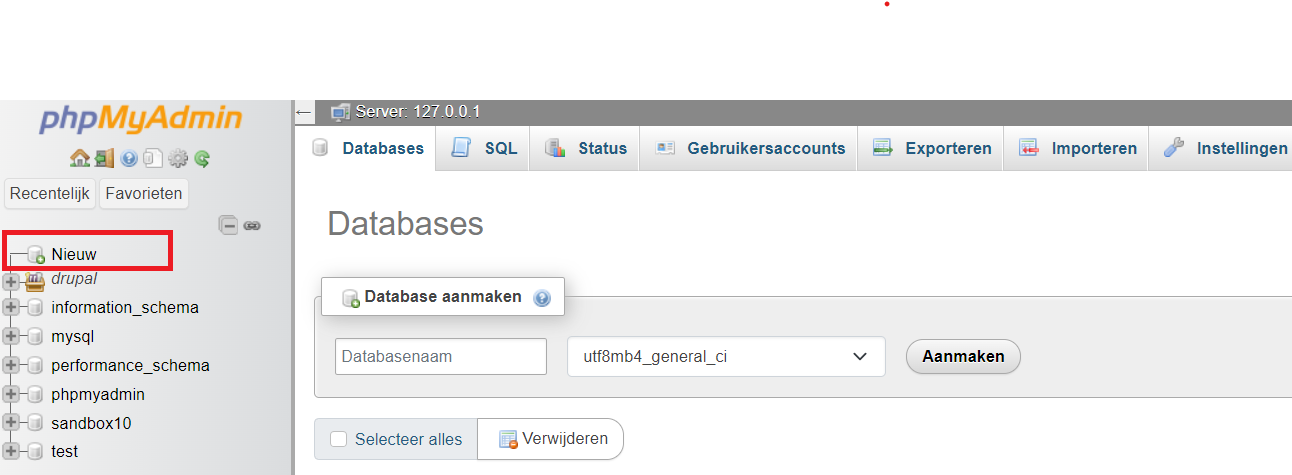
\includegraphics[width=1\linewidth]{img/ch3/createDB}
    \caption{You can manage your databases via phpMyAdmin}
    \label{fig:db_create}
\end{figure}

\section{Install Drupal}
Now that everything is in place, we can browse to our new website and start the installation process.

Using XAMPP, you can find your websites by navigating to https://localhost/<site-folder>. For example, if we use composer to create a new website in de htdocs folder, with the name newssite, we can browse to https://localhost/newssite.

From here, we can navigate to the web folder, which holds our index.php file and is our entry point to the website.

Now we are shown the installation screen where we need to select the language to install Drupal in. We'll choose 'English' and click 'Save and continue'.

\begin{figure}[h]
    \centering
    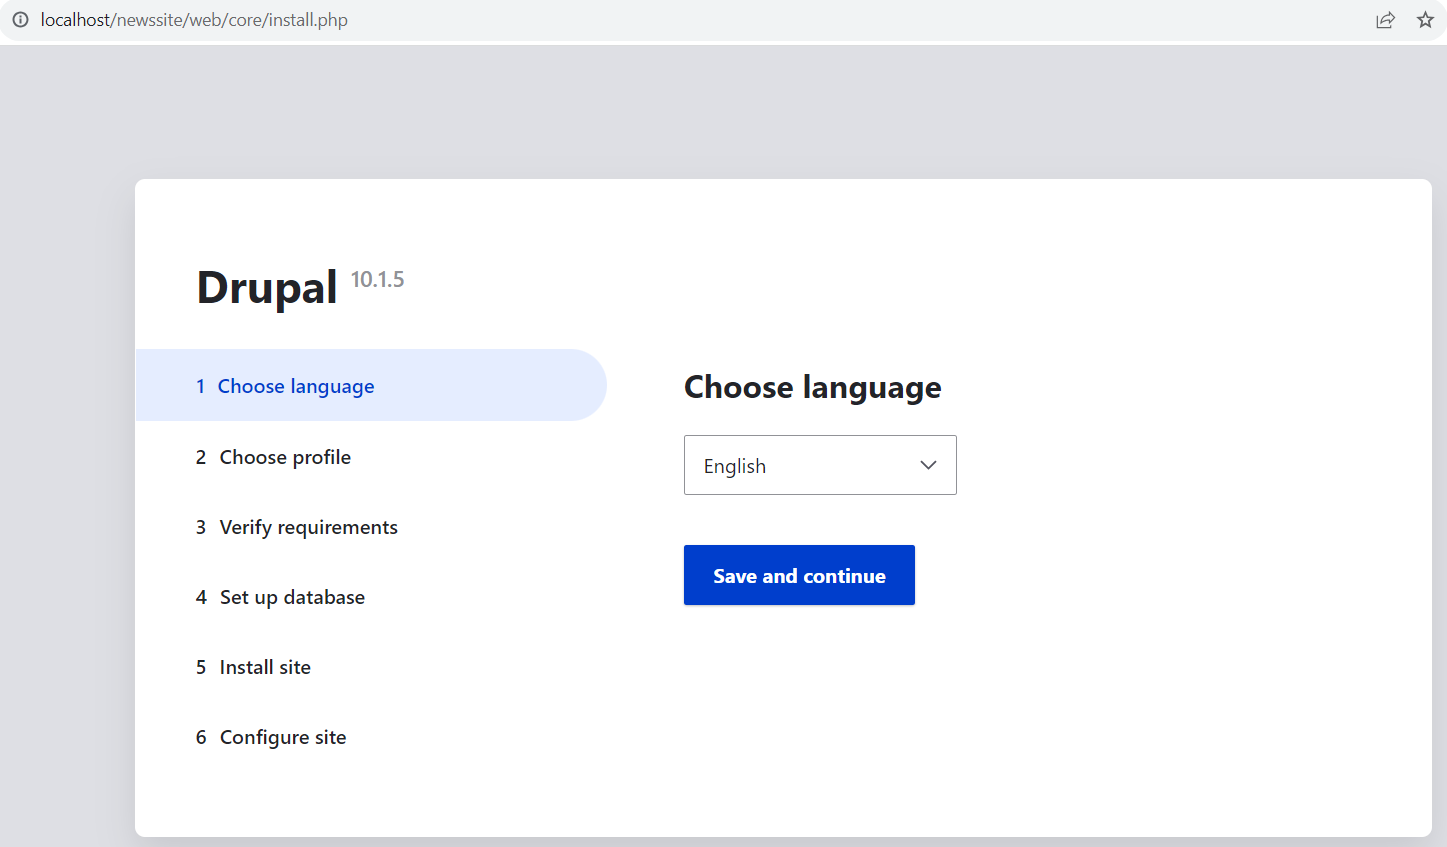
\includegraphics[width=1\linewidth]{img/ch3/install_step1}
    \caption{Follow the installation wizard to install a fresh Drupal website}
    \label{fig:install_step1}
\end{figure}

Next we'll stick with the standard installation and in step 3 Drupal shows us the requirements to continue the installation. We can ignore warnings, but errors need to be fixed. Drupal always provides information what's wrong, and how to fix it. At the bottom of the page we can click 'continue anyways' to ignore the warnings and continue the installation.

\begin{figure}[h]
    \centering
    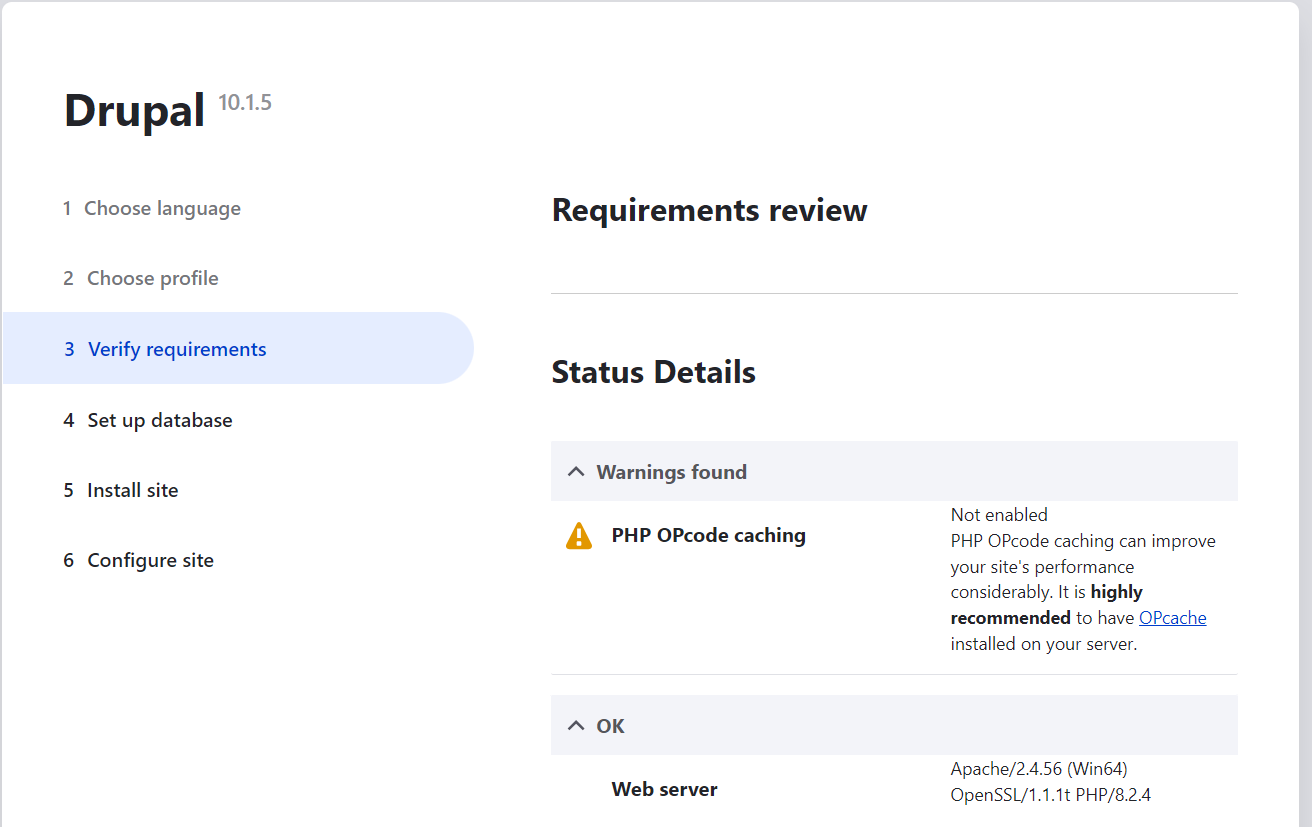
\includegraphics[width=1\linewidth]{img/ch3/install_step3}
    \caption{An overview of the minimum requirements to install Drupal}
    \label{fig:install_step3}
\end{figure}

In step 4, we need to enter the details of the database we created earlier. In our example, the database name is 'drupal\textunderscore newssite'. The database username and password depend on your installation. The default is set to 'root' as username without any password. But this can differ from your set up. If your database is running on a different server and or port, you can change it in the advanced options section.

\begin{figure}[h]
    \centering
    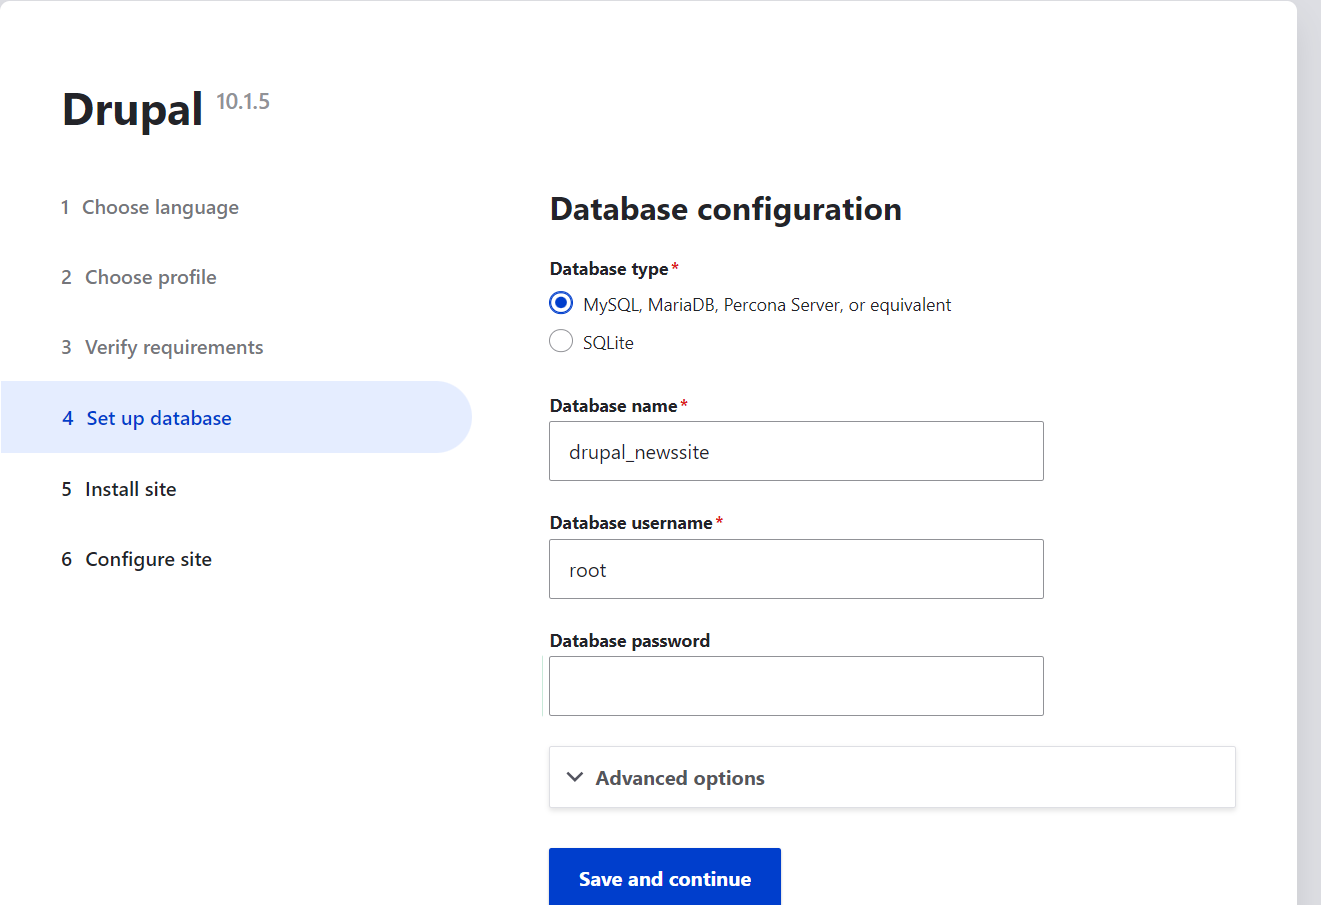
\includegraphics[width=1\linewidth]{img/ch3/install_step4}
    \caption{Setup the connection to the database}
    \label{fig:install_step4}
\end{figure}

Drupal continues to install the website and connect to the database to store all necessary data. In step 6, we finish up by entering some website details. These can be changed later in the administration tools as well.

\begin{figure}[h]
    \centering
    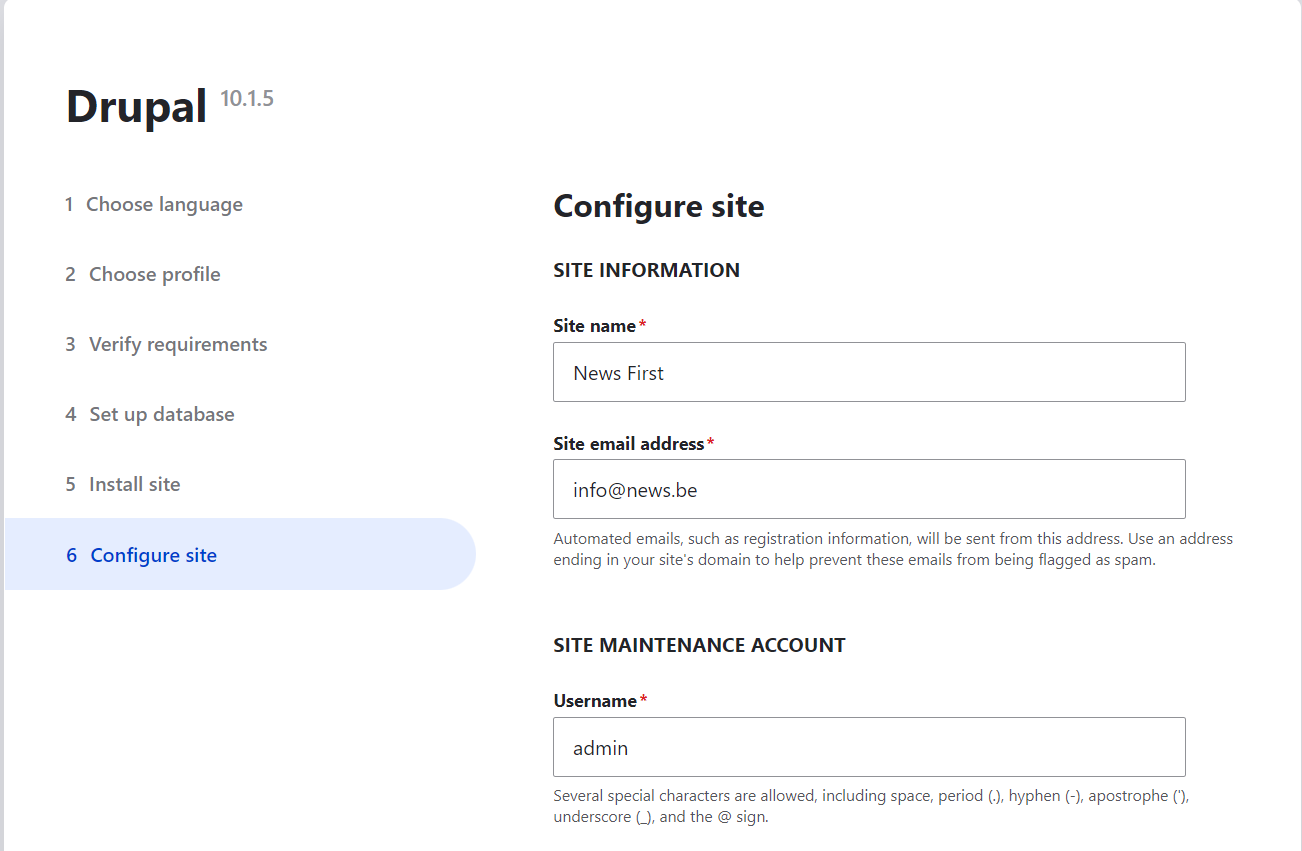
\includegraphics[width=1\linewidth]{img/ch3/install_step6}
    \caption{Enter the site details}
    \label{fig:install_step6}
\end{figure}

For our site we'll fill in the following details:
\begin{itemize}
    \item Site name: News First
    \item Site email address: info@news.be
    \item Username: admin
    \item Password: drupal
    \item Select your regional settings
    \item Untick the box 'Receive email notifications'. Seeing this is a sample site, this is not necessary.
\end{itemize}


\begin{figure}[h]
    \centering
    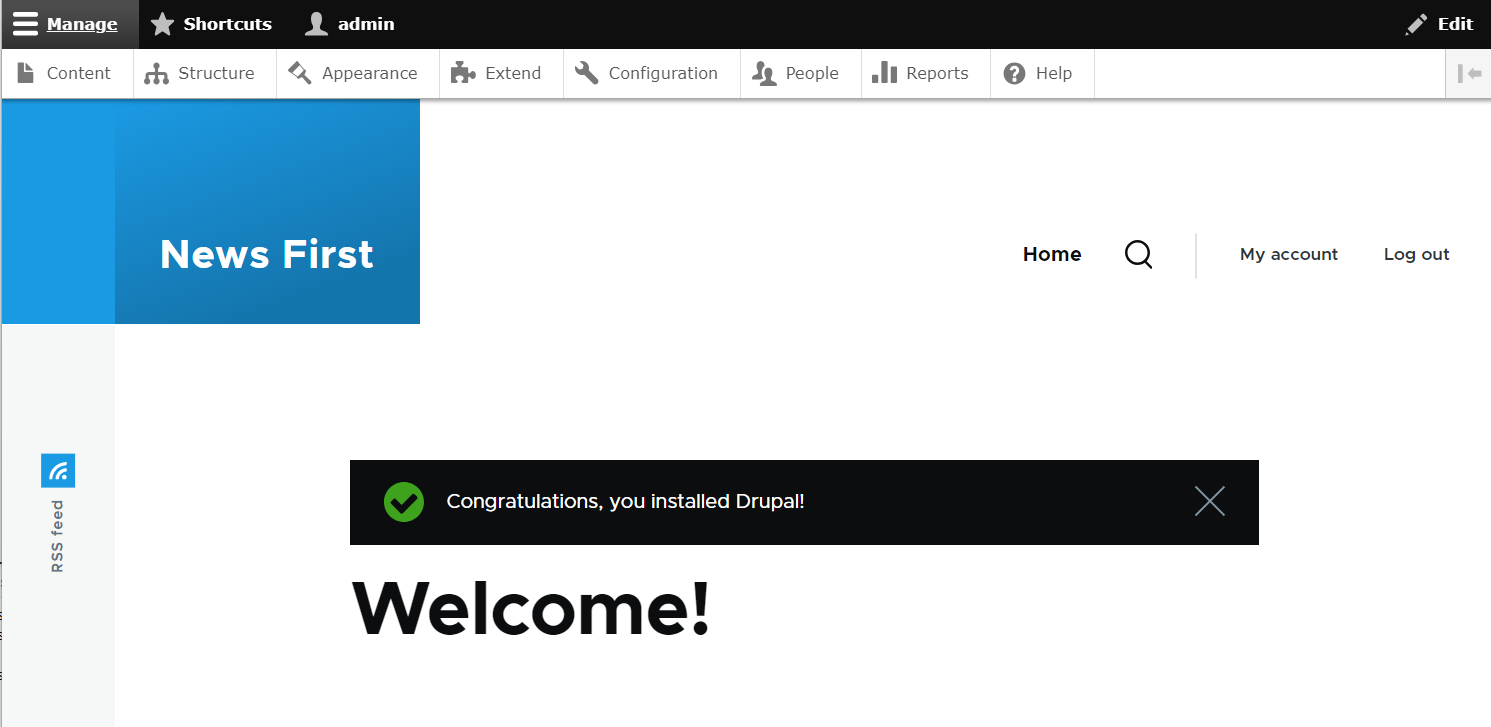
\includegraphics[width=1\linewidth]{img/ch3/install_complete}
    \caption{A fresh Drupal website}
    \label{fig:install_complete}
\end{figure}

Et voila, you have your first Drupal site. It’s pretty basic, you only have a welcome page, no content yet. By default, after completing the installation, you are logged in as administrator. To see the non-administrator layout, click the Log out link in the top right corner. As you can see, we only have a basic one-page site with our site title at the top. Now log back into your site with username: admin and password: drupal.

\section{Review exercise}

Create a new Drupal site with the following properties:
\begin{itemize}
    \item Site name: bitingbugsexample
    \item Site email address: noreply@bitingbugsexample.com
    \item Username: admin
    \item Password: drupal
    \item Email address: info@bitingbugsexample.com
    \item Default country: Belgium
    \item Default time zone: Europe/Brussels  
\end{itemize}







